\documentclass[aspectratio=169]{beamer}
\setbeamertemplate{navigation symbols}{}
\usepackage{color, amsmath, comment, subfigure}
\usepackage{url}

\usepackage{hyperref}
\hypersetup{
    colorlinks=true,
    linkcolor=blue,
    filecolor=magenta,      
    urlcolor=cyan,
}

%%%%%%%%%%%%%%%%%%%%%%%%%%
\title[]{Pre-read for Tuesday, October 6:\\Social fads, part 1}
\author[]{Matthew J. Salganik}
\institute[]{}
\date[]{COS 597E/SOC 555 Limits to prediction\\Fall 2020, Princeton University}

\begin{document}
%%%%%%%%%%%%%%%%%%%%%%%%%%%
\frame{\titlepage}
%%%%%%%%%%%%%%%%%%%%%%%%%%%
\begin{frame}

\begin{center}
  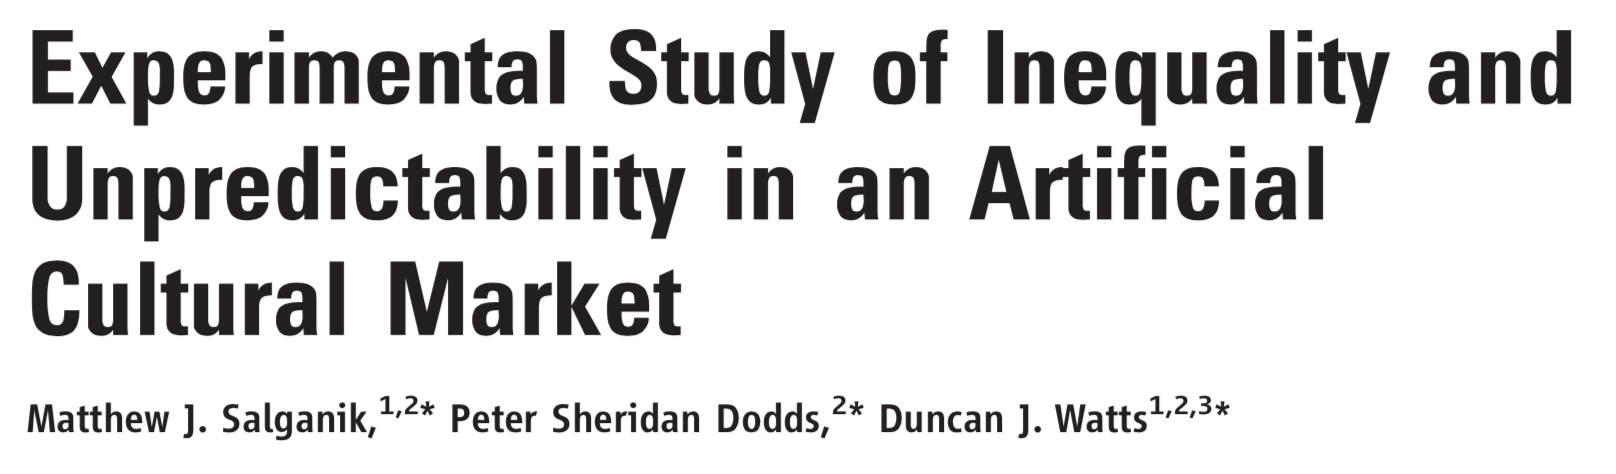
\includegraphics[width = 0.9\textwidth]{figures/salganik_experimental_2006_title}
\end{center}

\end{frame}
%%%%%%%%%%%%%%%%%%%%%%%%%%%
\begin{frame}

  \begin{columns}
    \column{0.4\textwidth}
     \begin{block}{}
       
\includegraphics[width=\textwidth]{figures/hp-cover.pdf}
     \end{block}

   \pause
   
   \column{0.6\textwidth}
     \begin{block}{}
       \begin{itemize}
         \item Wild success
         \item Rejected by eight publishers\\
       \end{itemize}
       This seems like a strange combination.
     \end{block}
  \end{columns}

\end{frame}
%%%%%%%%%%%%%%%%%%%%%%%%
\begin{frame}

  \begin{columns}
    \column{0.4\textwidth}
     \begin{block}{}
       
\includegraphics[width=\textwidth]{figures/star-wars}
     \end{block}
   
   \column{0.6\textwidth}
     \begin{block}{}
       \begin{itemize}
         \item Set box office records, won 6 Oscars, and launched a multi-billion dollar franchise
         \item Rejected by United Artists and Universal before being made by Fox
       \end{itemize}
     \end{block}
  \end{columns}

\end{frame}
%%%%%%%%%%%%
\begin{frame}

  \begin{columns}
    \column{0.4\textwidth}
     \begin{block}{}
       
\includegraphics[width=\textwidth]{figures/american-idol}
     \end{block}

   \column{0.6\textwidth}
     \begin{block}{}
       \begin{itemize}
         \item One of the most popular shows of the decade
         \item Rejected by ABC, CBS, and NBC before being picked up by Fox
       \end{itemize}
     \end{block}
  \end{columns}

\end{frame}

%%%%%%%%%%%%%%%%
\begin{frame}

  Puzzling nature of success for cultural objects (books, movies, piece of art, music, TV shows)
  \vspace{0.2in}
  \begin{itemize}
    \item<1-> {\bf extreme inequality in the success of objects} \\
    \item <2->{\bf unpredictability in the success of objects} \\
  \end{itemize}

\end{frame}
%%%%%%%%%%%%%%%%%%%%%%%%%%%%%%%
\begin{frame} 

\textbf{Psychological explanation:}\\
People agree on what's good, but people are hard to predict\\

\pause
\vspace{0.2in}

\textbf{Sociological explanation:}\\
The collective outcomes of inequality and unpredictability of success both arise from an individual-level process of social influence\\

\begin{figure}
  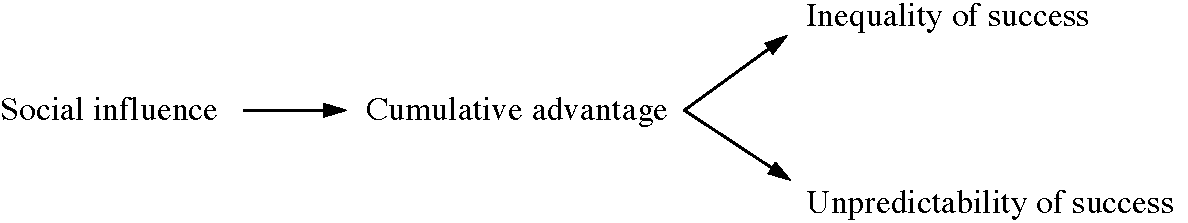
\includegraphics[width = 0.8\textwidth]{figures/musiclab_model}
\end{figure}

\end{frame}

%%%%%%%%%%%%%%%%%%%%%%%%%%%%%%%%%%%
\begin{frame}

\begin{figure}
  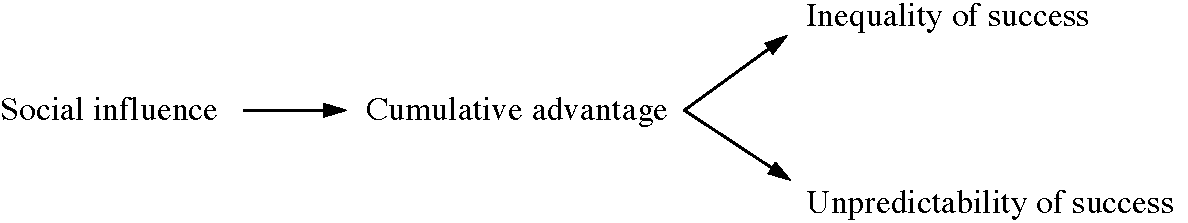
\includegraphics[width = 0.8\textwidth]{figures/musiclab_model}
\end{figure}

Problems with observational data:
\begin{itemize}
\item don't know what would have happened without social influence
\item can't see multiple ``histories'' to observe unpredictability
\end{itemize}

\end{frame}

%%%%%%%%%%%%%%%%%%%%%%%%%%%%%%%%%%%
\begin{frame}

Instead of using observational data we are going to run an experiment because
\begin{itemize}
\item can run the same process multiple times under exactly the same conditions, allows us to see multiple ``histories''
\item can control the information that people have about the behavior of others
\end{itemize}

\pause
\vspace{0.2in}
But, this experiment is different from most,
\begin{itemize}
\item experiments in psychology and economics have \textbf{individual} as unit of analysis, require \textbf{hundreds} of participants 
\item these sociological experiments have \textbf{collective outcome} as unit of analysis, require \textbf{thousands} of participants
\end{itemize}
Web-based experiment allow for such large sample sizes because each additional participant has no cost (total $n= 27,267$)\\

\end{frame}
%%%%%%%%%%%%%%%%%%%%%%%%%%%%%%%%%%%
\begin{frame}

\begin{center}
\includegraphics<1>[width = 0.85\textwidth]{figures/zero_variable_cost_1}
\includegraphics<2>[width = 0.85\textwidth]{figures/zero_variable_cost_2}
\end{center}

\end{frame}
%%%%%%%%%%%%%%%%%%%%%%%%%%%%
\begin{frame}

\begin{figure}
  \centering
  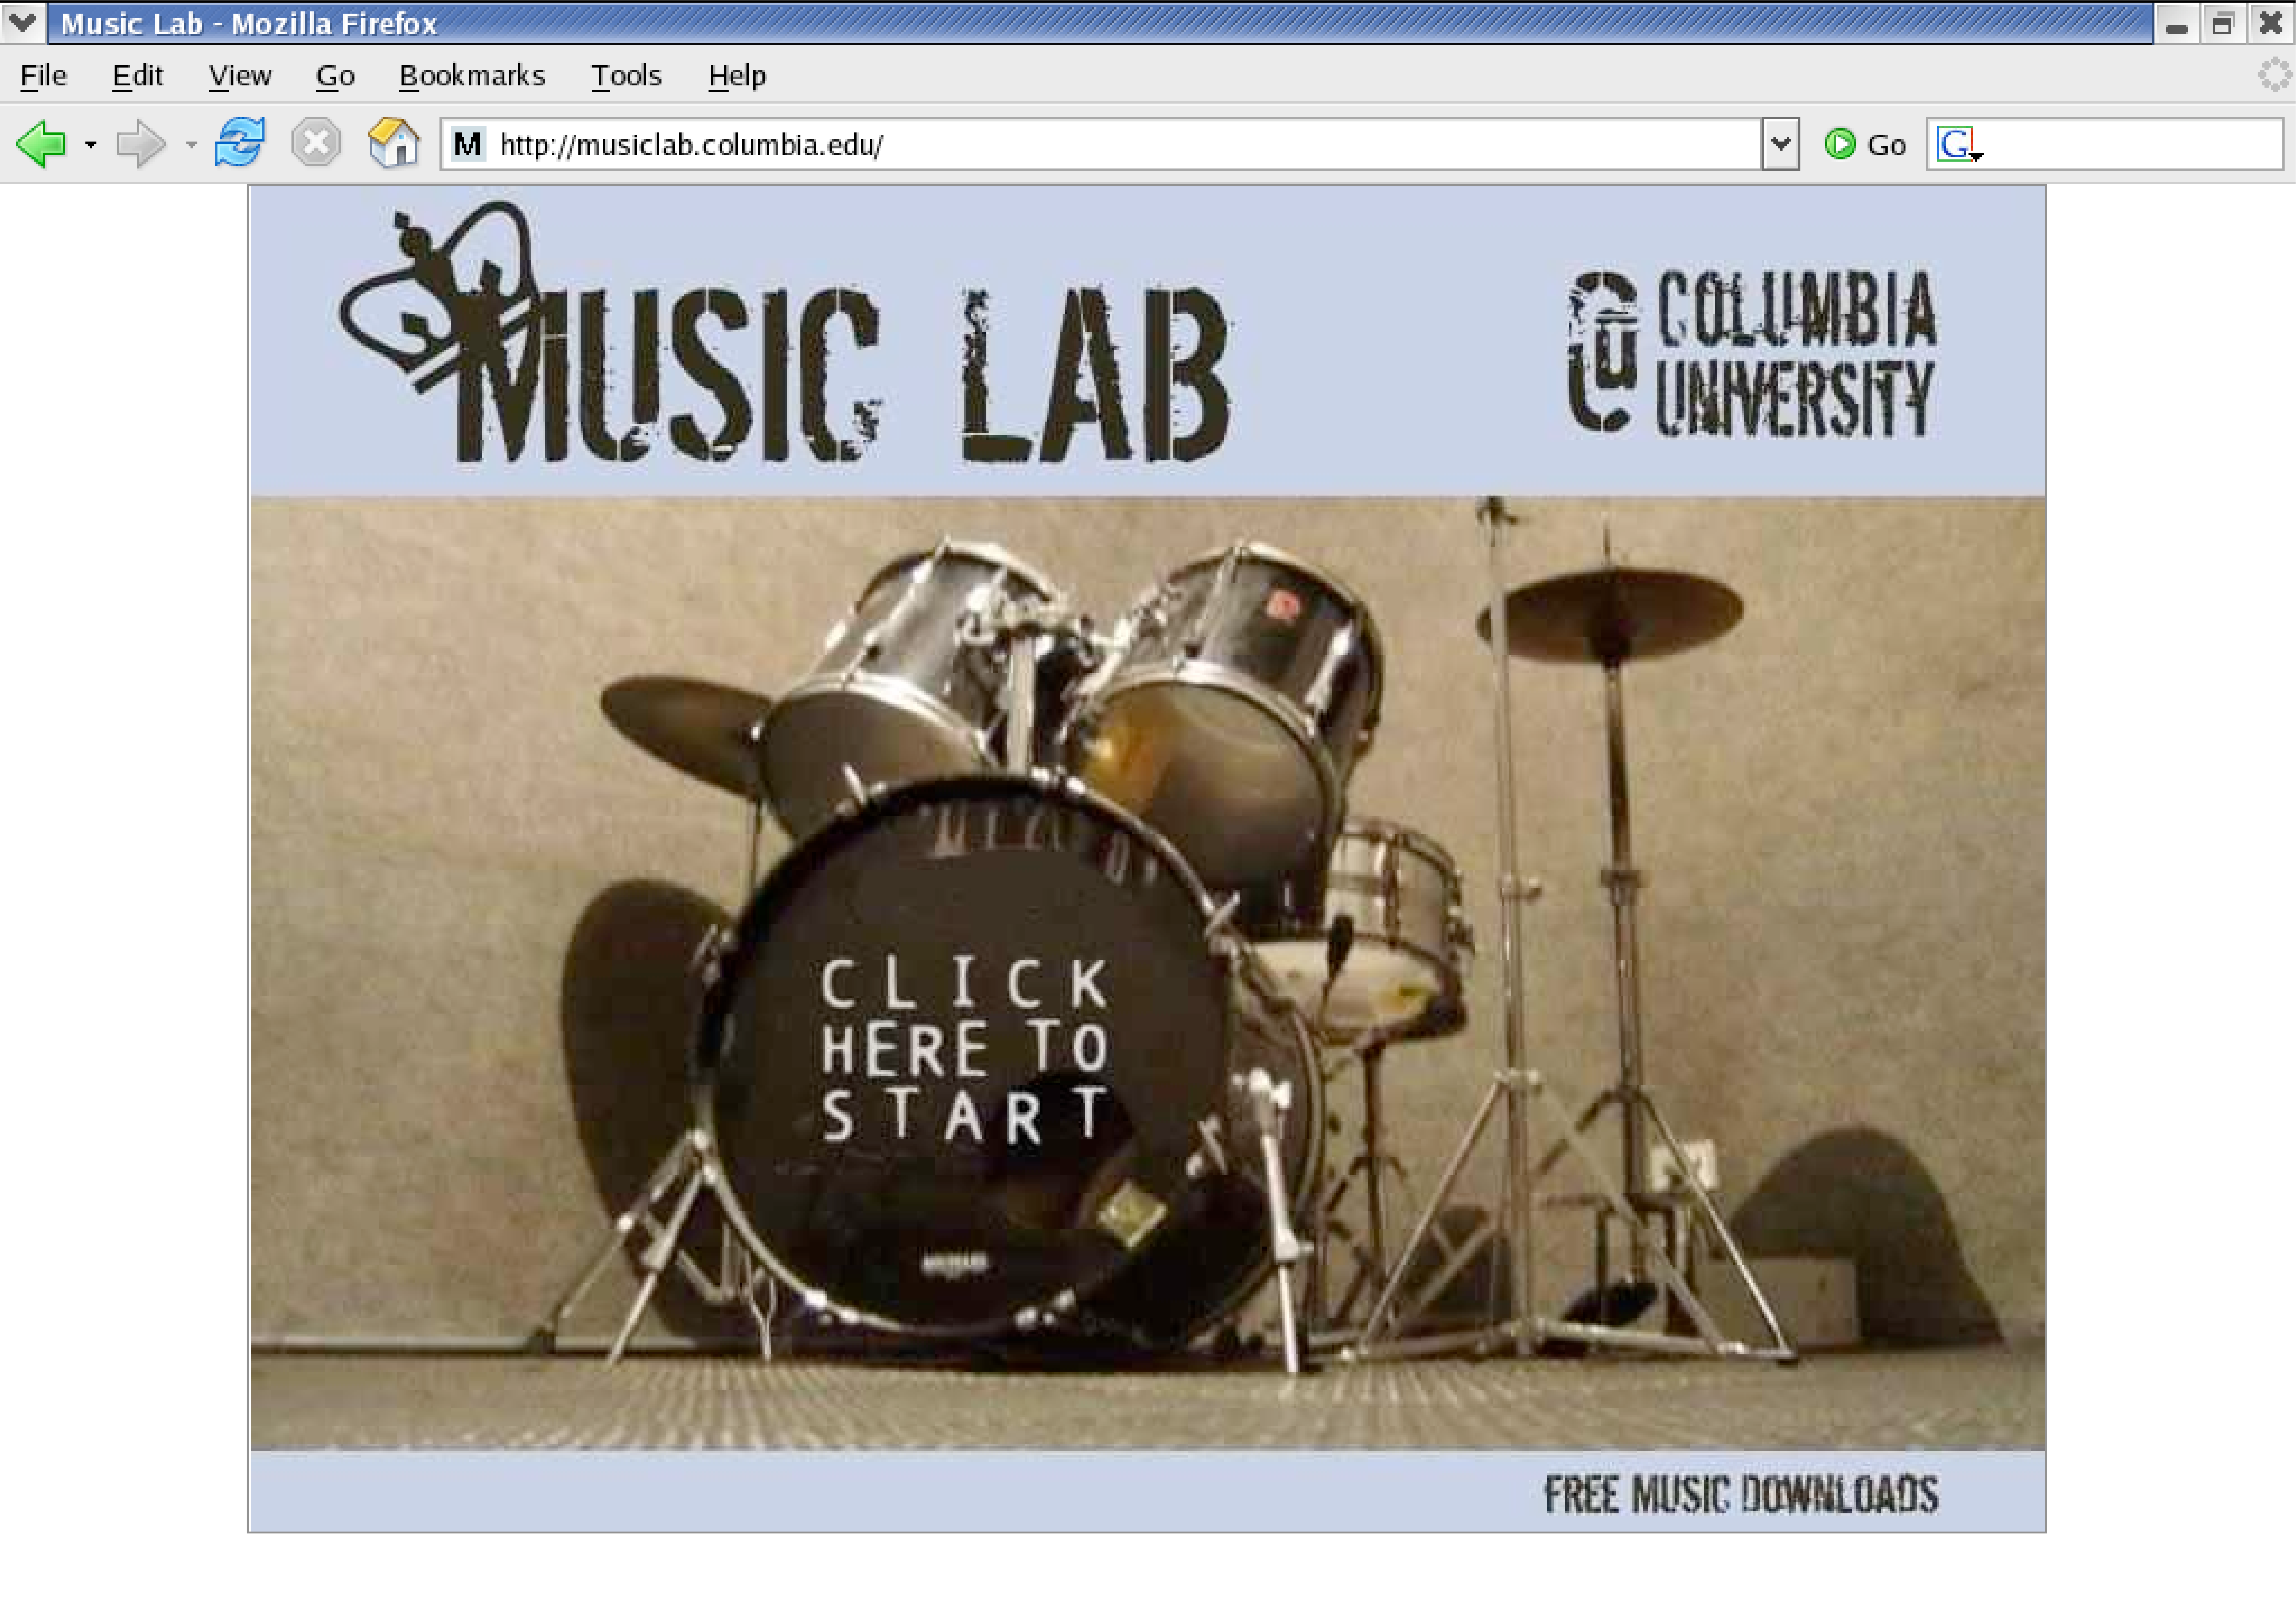
\includegraphics[width = 0.9\textwidth]{figures/splashscreen}
\end{figure}

\end{frame}
%%%%%%%%%%%%%%%%%%%%%%%%%%%%%%%%%
\begin{frame}

\begin{figure}
  \centering
  \includegraphics[width = 0.9\textwidth]{figures/info-v1-cut}
\end{figure}

\end{frame}
%%%%%%%%%%%%%%%%%%%%%%%%%%%%%%%%%
\begin{frame} 

\begin{figure}
  \centering
  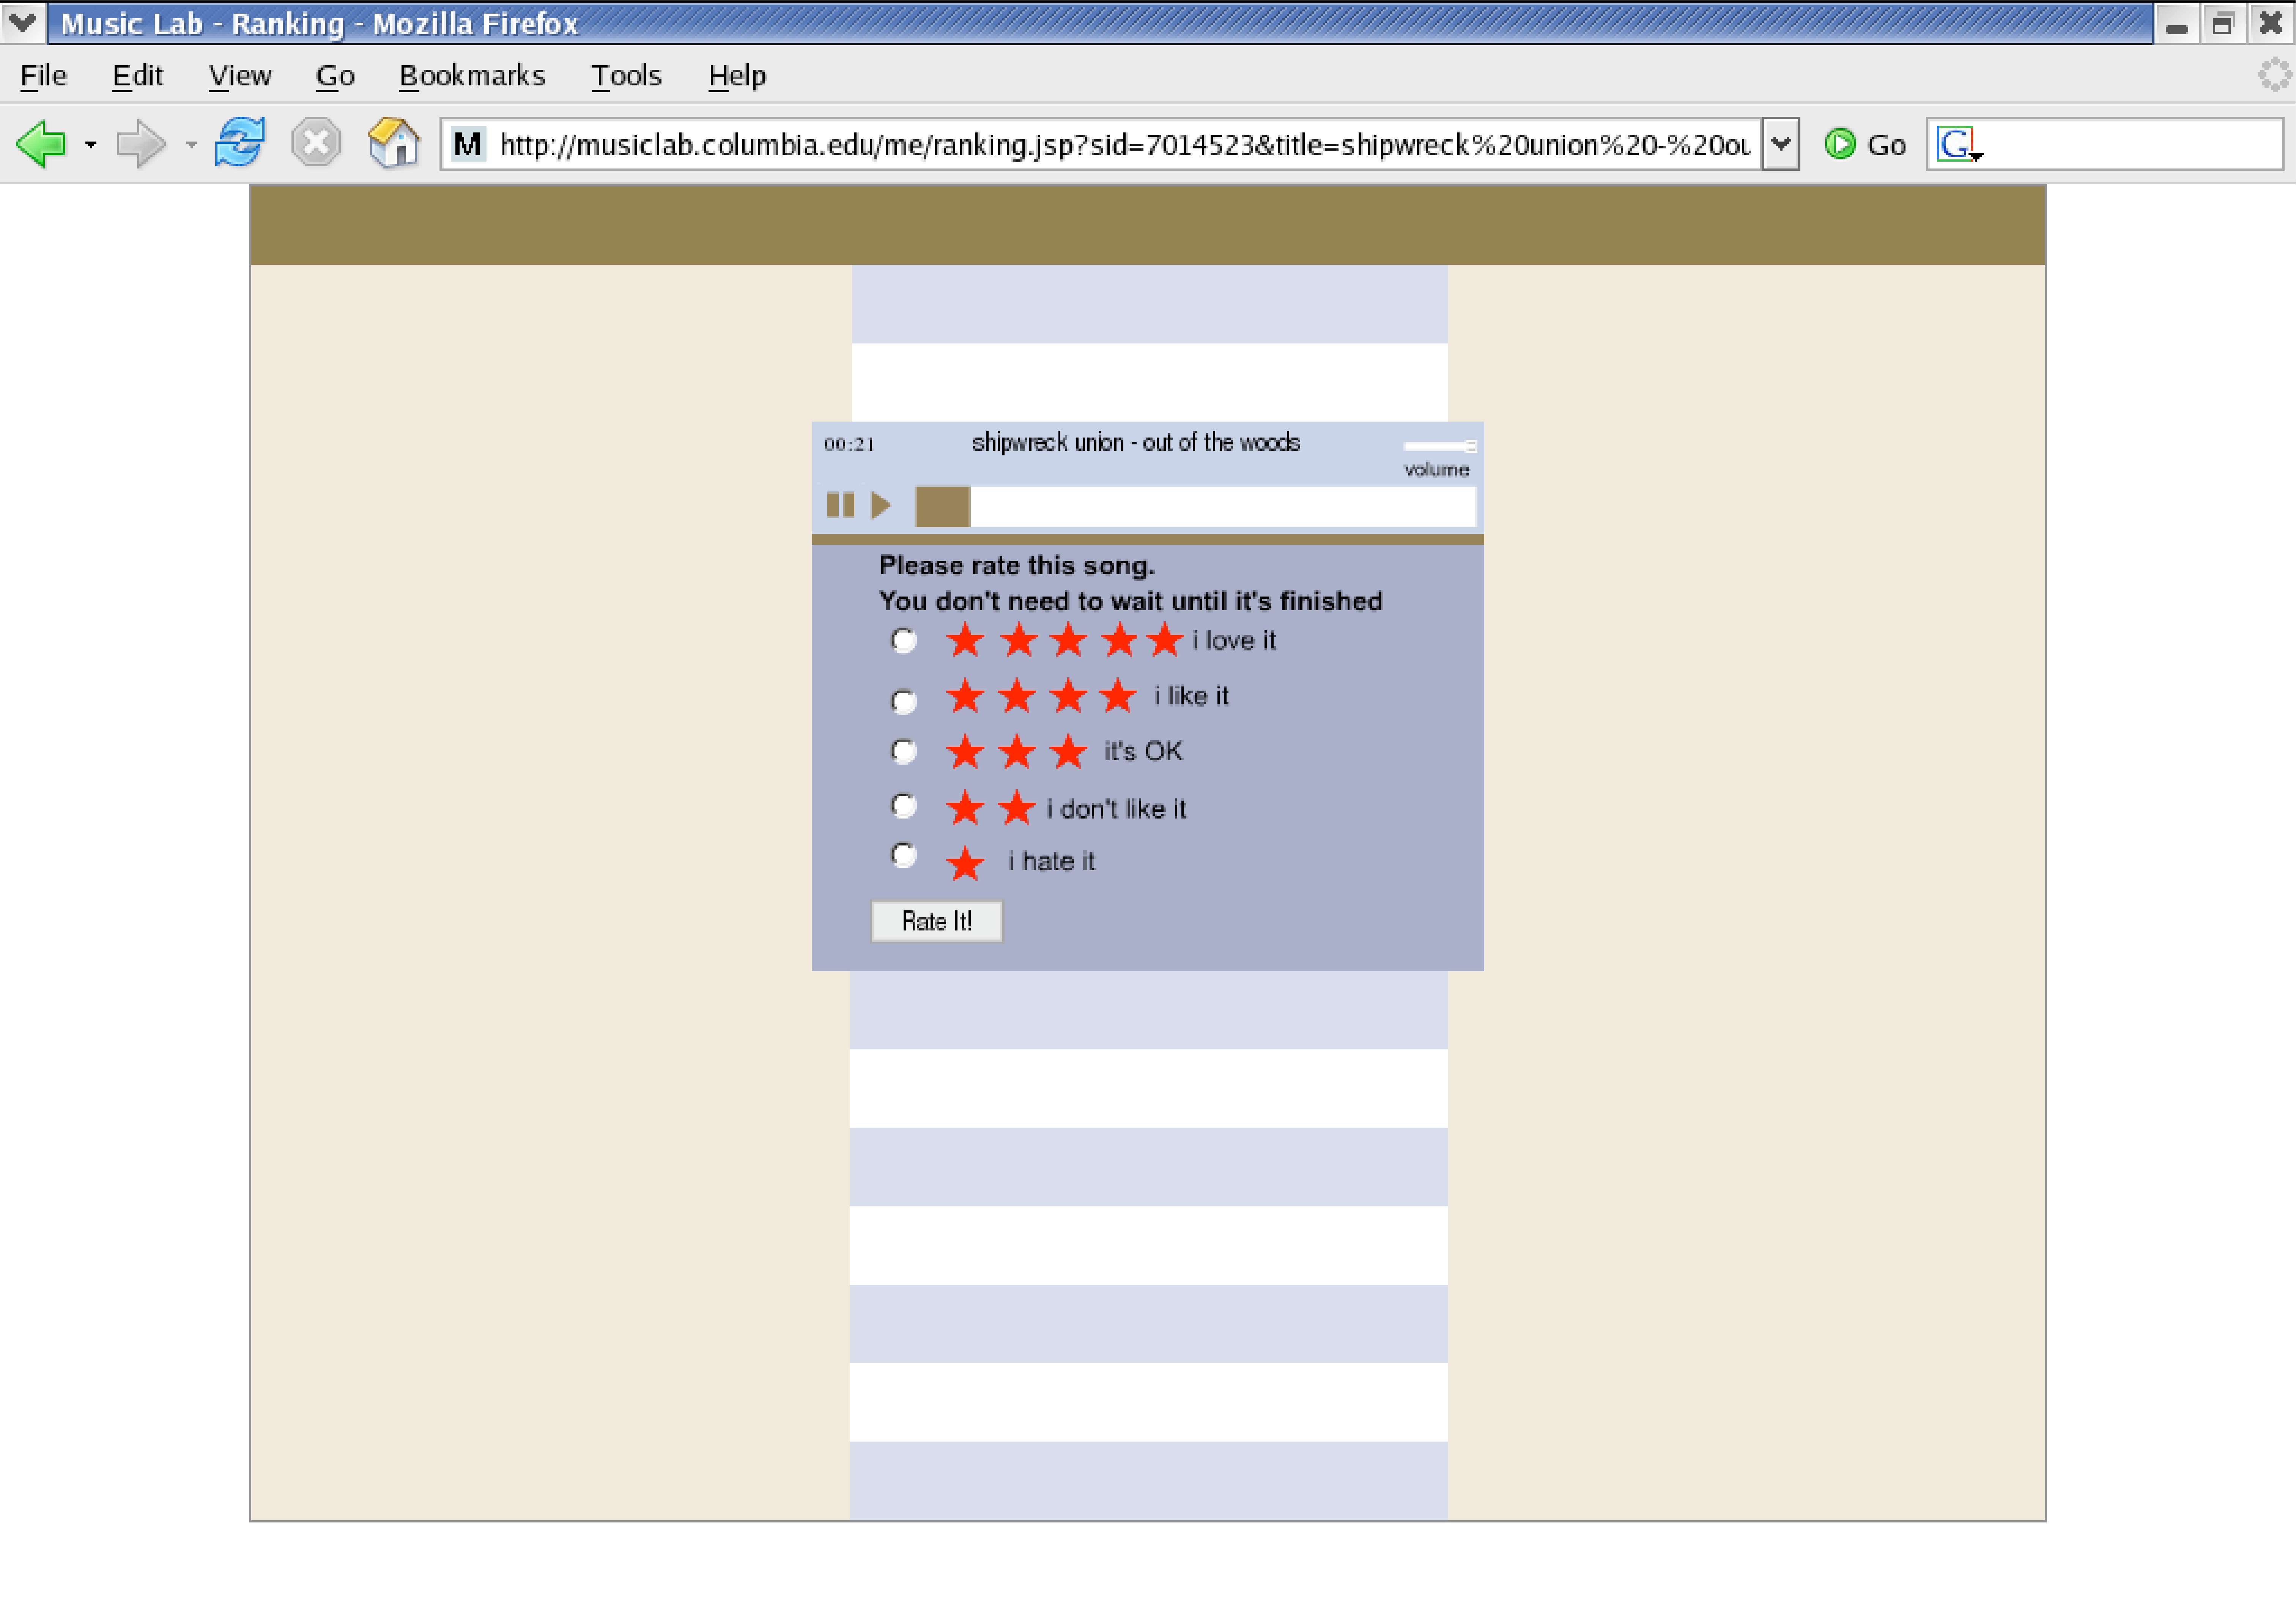
\includegraphics[width = 0.9\textwidth]{figures/listenscreen}
\end{figure}

\end{frame}
%%%%%%%%%%%%%%%%%%%%%%%%%%%%%%%%%
\begin{frame}

\begin{figure}
  \centering
  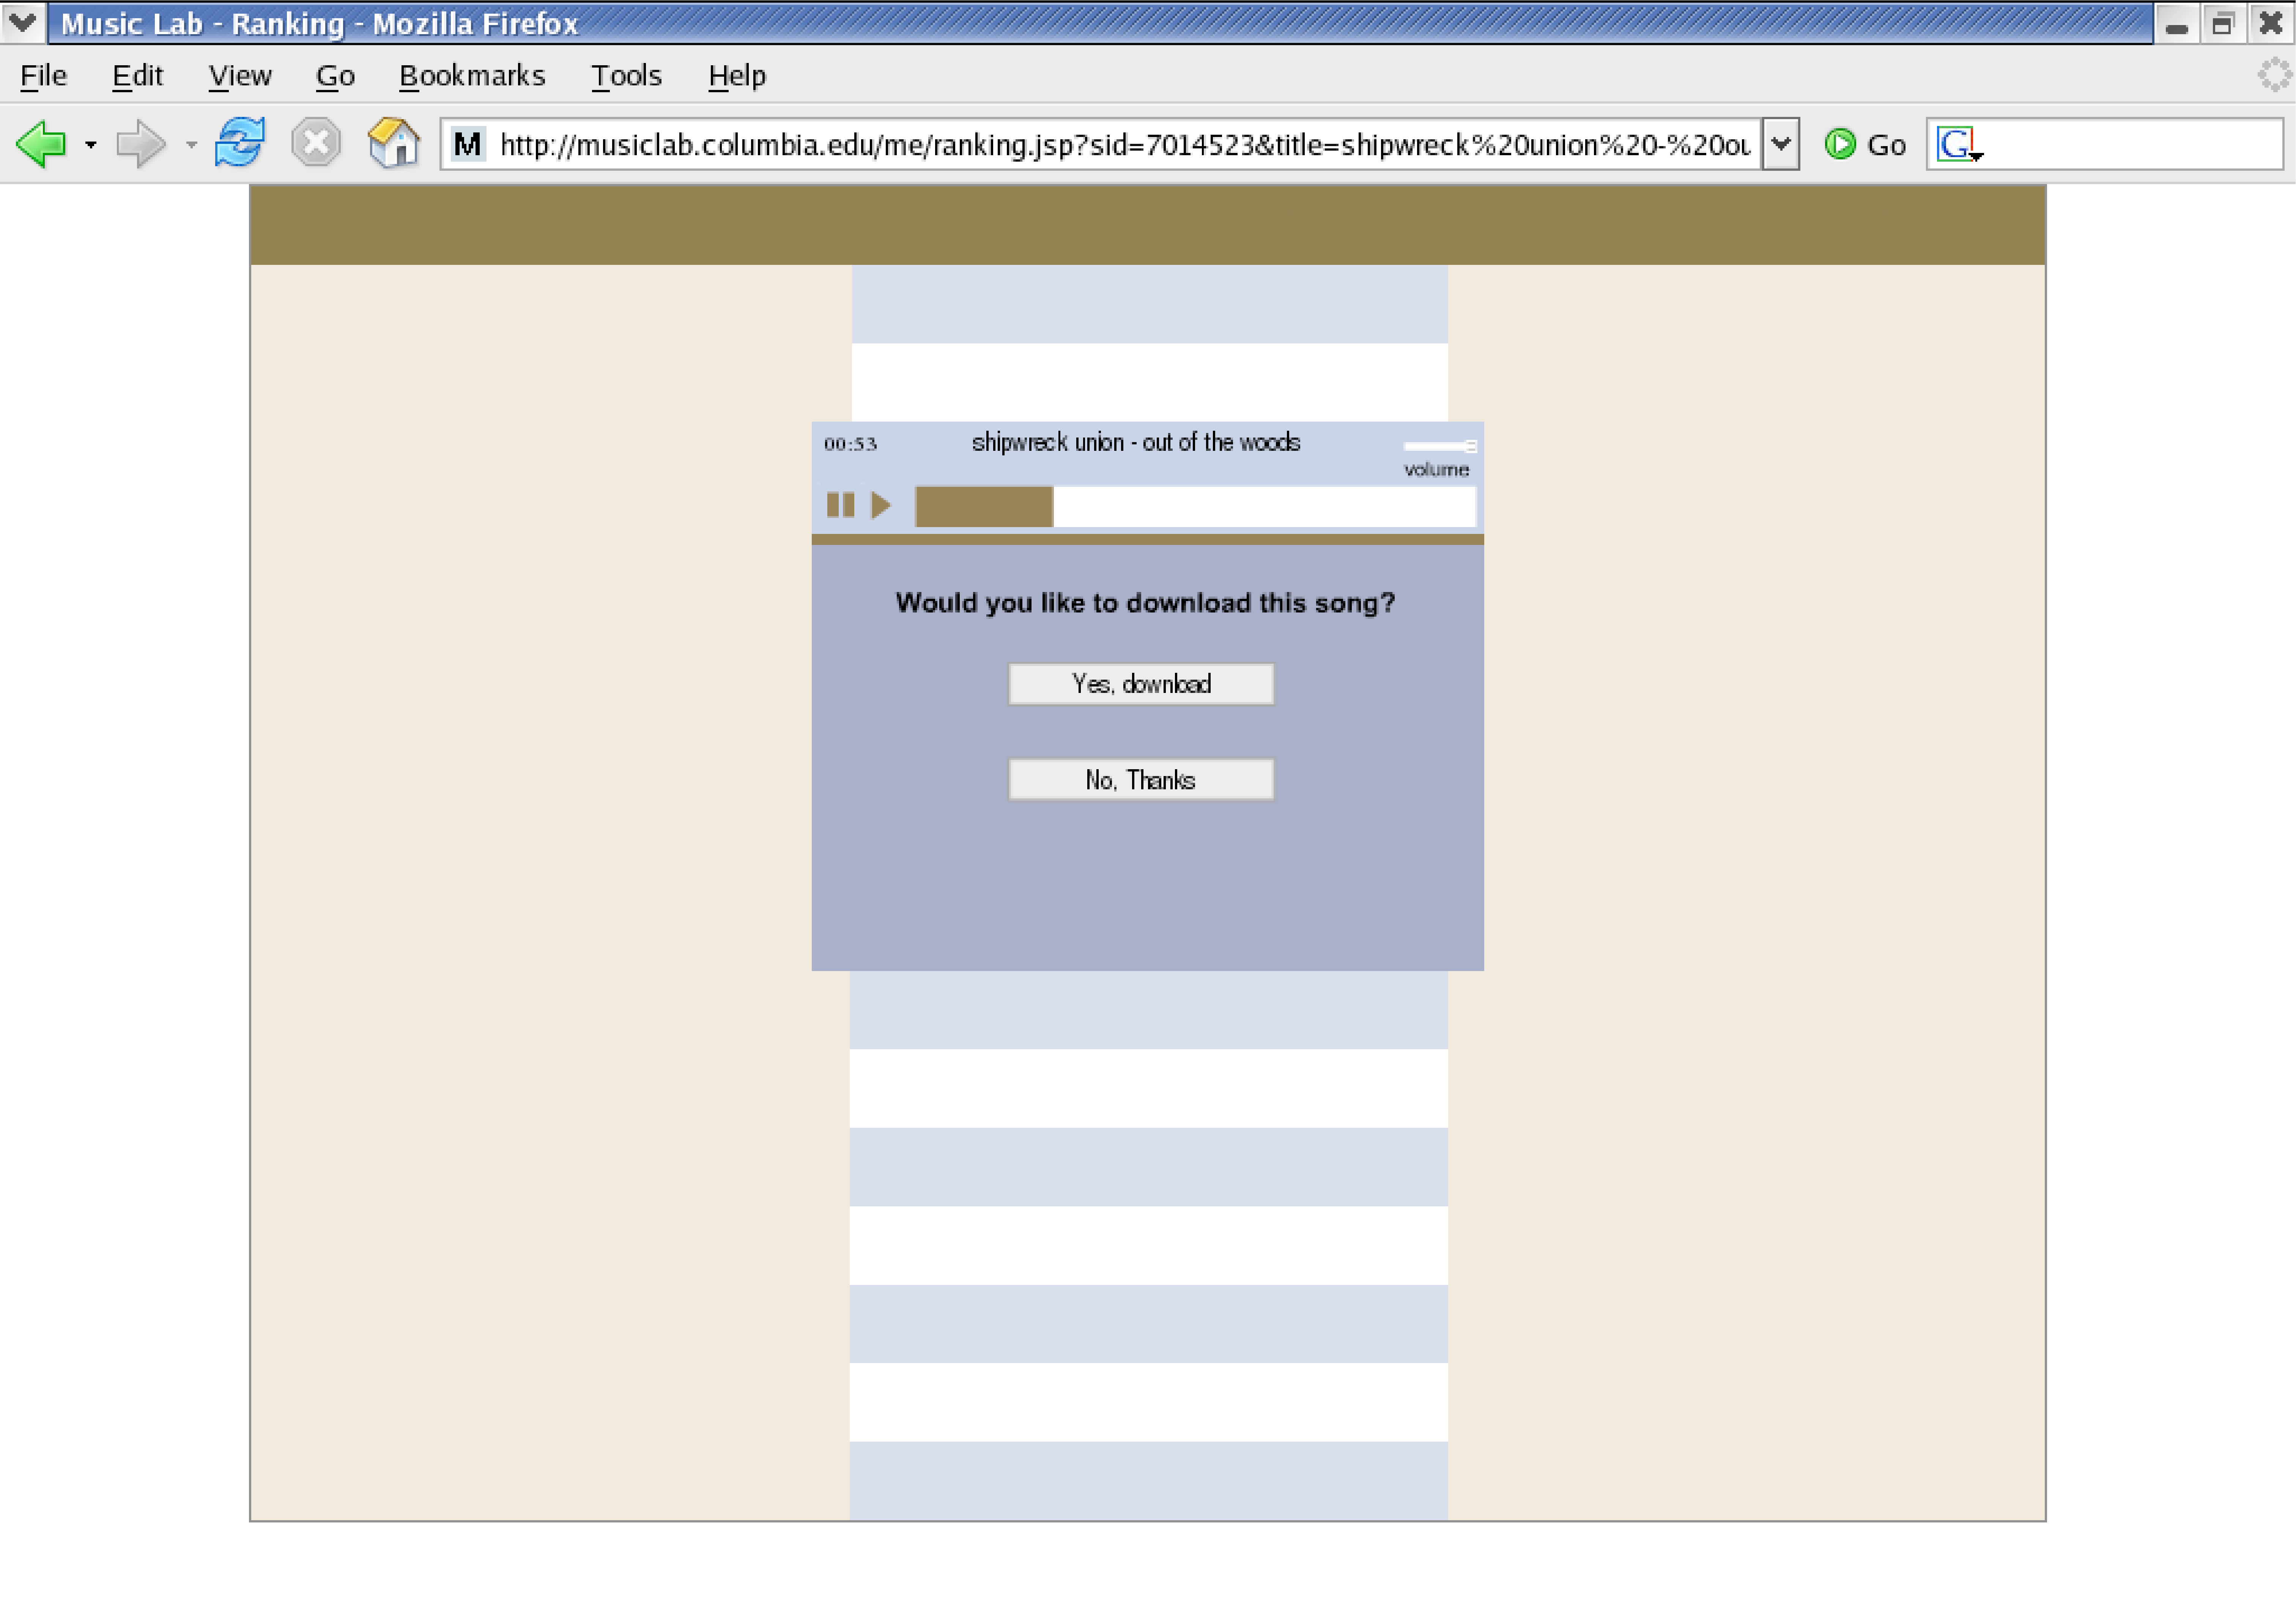
\includegraphics[width = 0.9\textwidth]{figures/downloadscreen}
\end{figure}

\end{frame}
%%%%%%%%%%%%%%%%%%%%%%%%%%%%%%%%%%
\begin{frame}

\begin{figure}
  \centering
  \includegraphics[width = 0.9\textwidth]{figures/info-v1-cut}
\end{figure}

\end{frame}
%%%%%%%%%%%%%%%%%%%%%%%%%%%%%%%%%
\begin{frame}

\begin{itemize}
\item \url{https://www.dropbox.com/s/k02iy1hcw0g3xir/165444-hi.mp3?dl=0}
\item \url{https://www.dropbox.com/s/j0wpjg379xuhe7n/331122-hi.mp3?dl=0}
\item \url{https://www.dropbox.com/s/tobqqk4ar9qzc01/846626-hi.mp3?dl=0}
\end{itemize}

\end{frame}
%%%%%%%%%%%%%%%%%%%%%%%%%%%%%%%%%
\begin{frame}

\begin{figure}
  \centering
  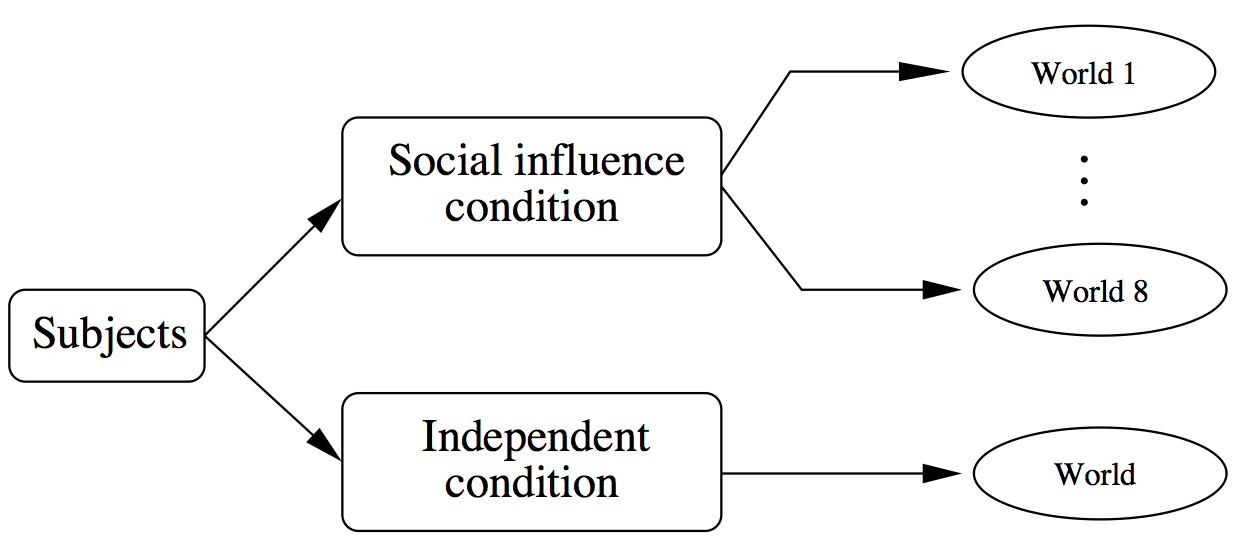
\includegraphics[width=0.9\textwidth]{figures/musiclab_exp_design}
\end{figure}

\end{frame}
%%%%%%%%%%%%%%%%%%%%%%%%%%%%%%%%%
%
%\begin{frame}
%\frametitle{Experiment 1: Screenshots}
%
%\setcounter{subfigure}{0}
%\begin{figure}
%  \centering
%     \subfigure[Social influence condition]{
%     \includegraphics[width=0.45\textwidth]{/Users/matt/projects/musiclab/screenshots/info-v1-cut.eps}}
%  \hspace{0in}
%    \subfigure[Independent condition]{
%     \includegraphics[width=0.45\textwidth]{/Users/matt/projects/musiclab/screenshots/noinfo-v1-cut.eps}}
%\end{figure}
%
%\end{frame}
%%%%%%%%%%%%%%%%%%%%%%%%%%%%%%%%%%
\begin{frame}

\setcounter{subfigure}{0}
\begin{figure}
  \centering
     \subfigure[Experiment 1, Weaker signal]{
     \includegraphics[width=0.45\textwidth]{figures/info-v1-cut}}
  \hspace{0in}
     \subfigure[Experiment 2, Stronger signal]{
     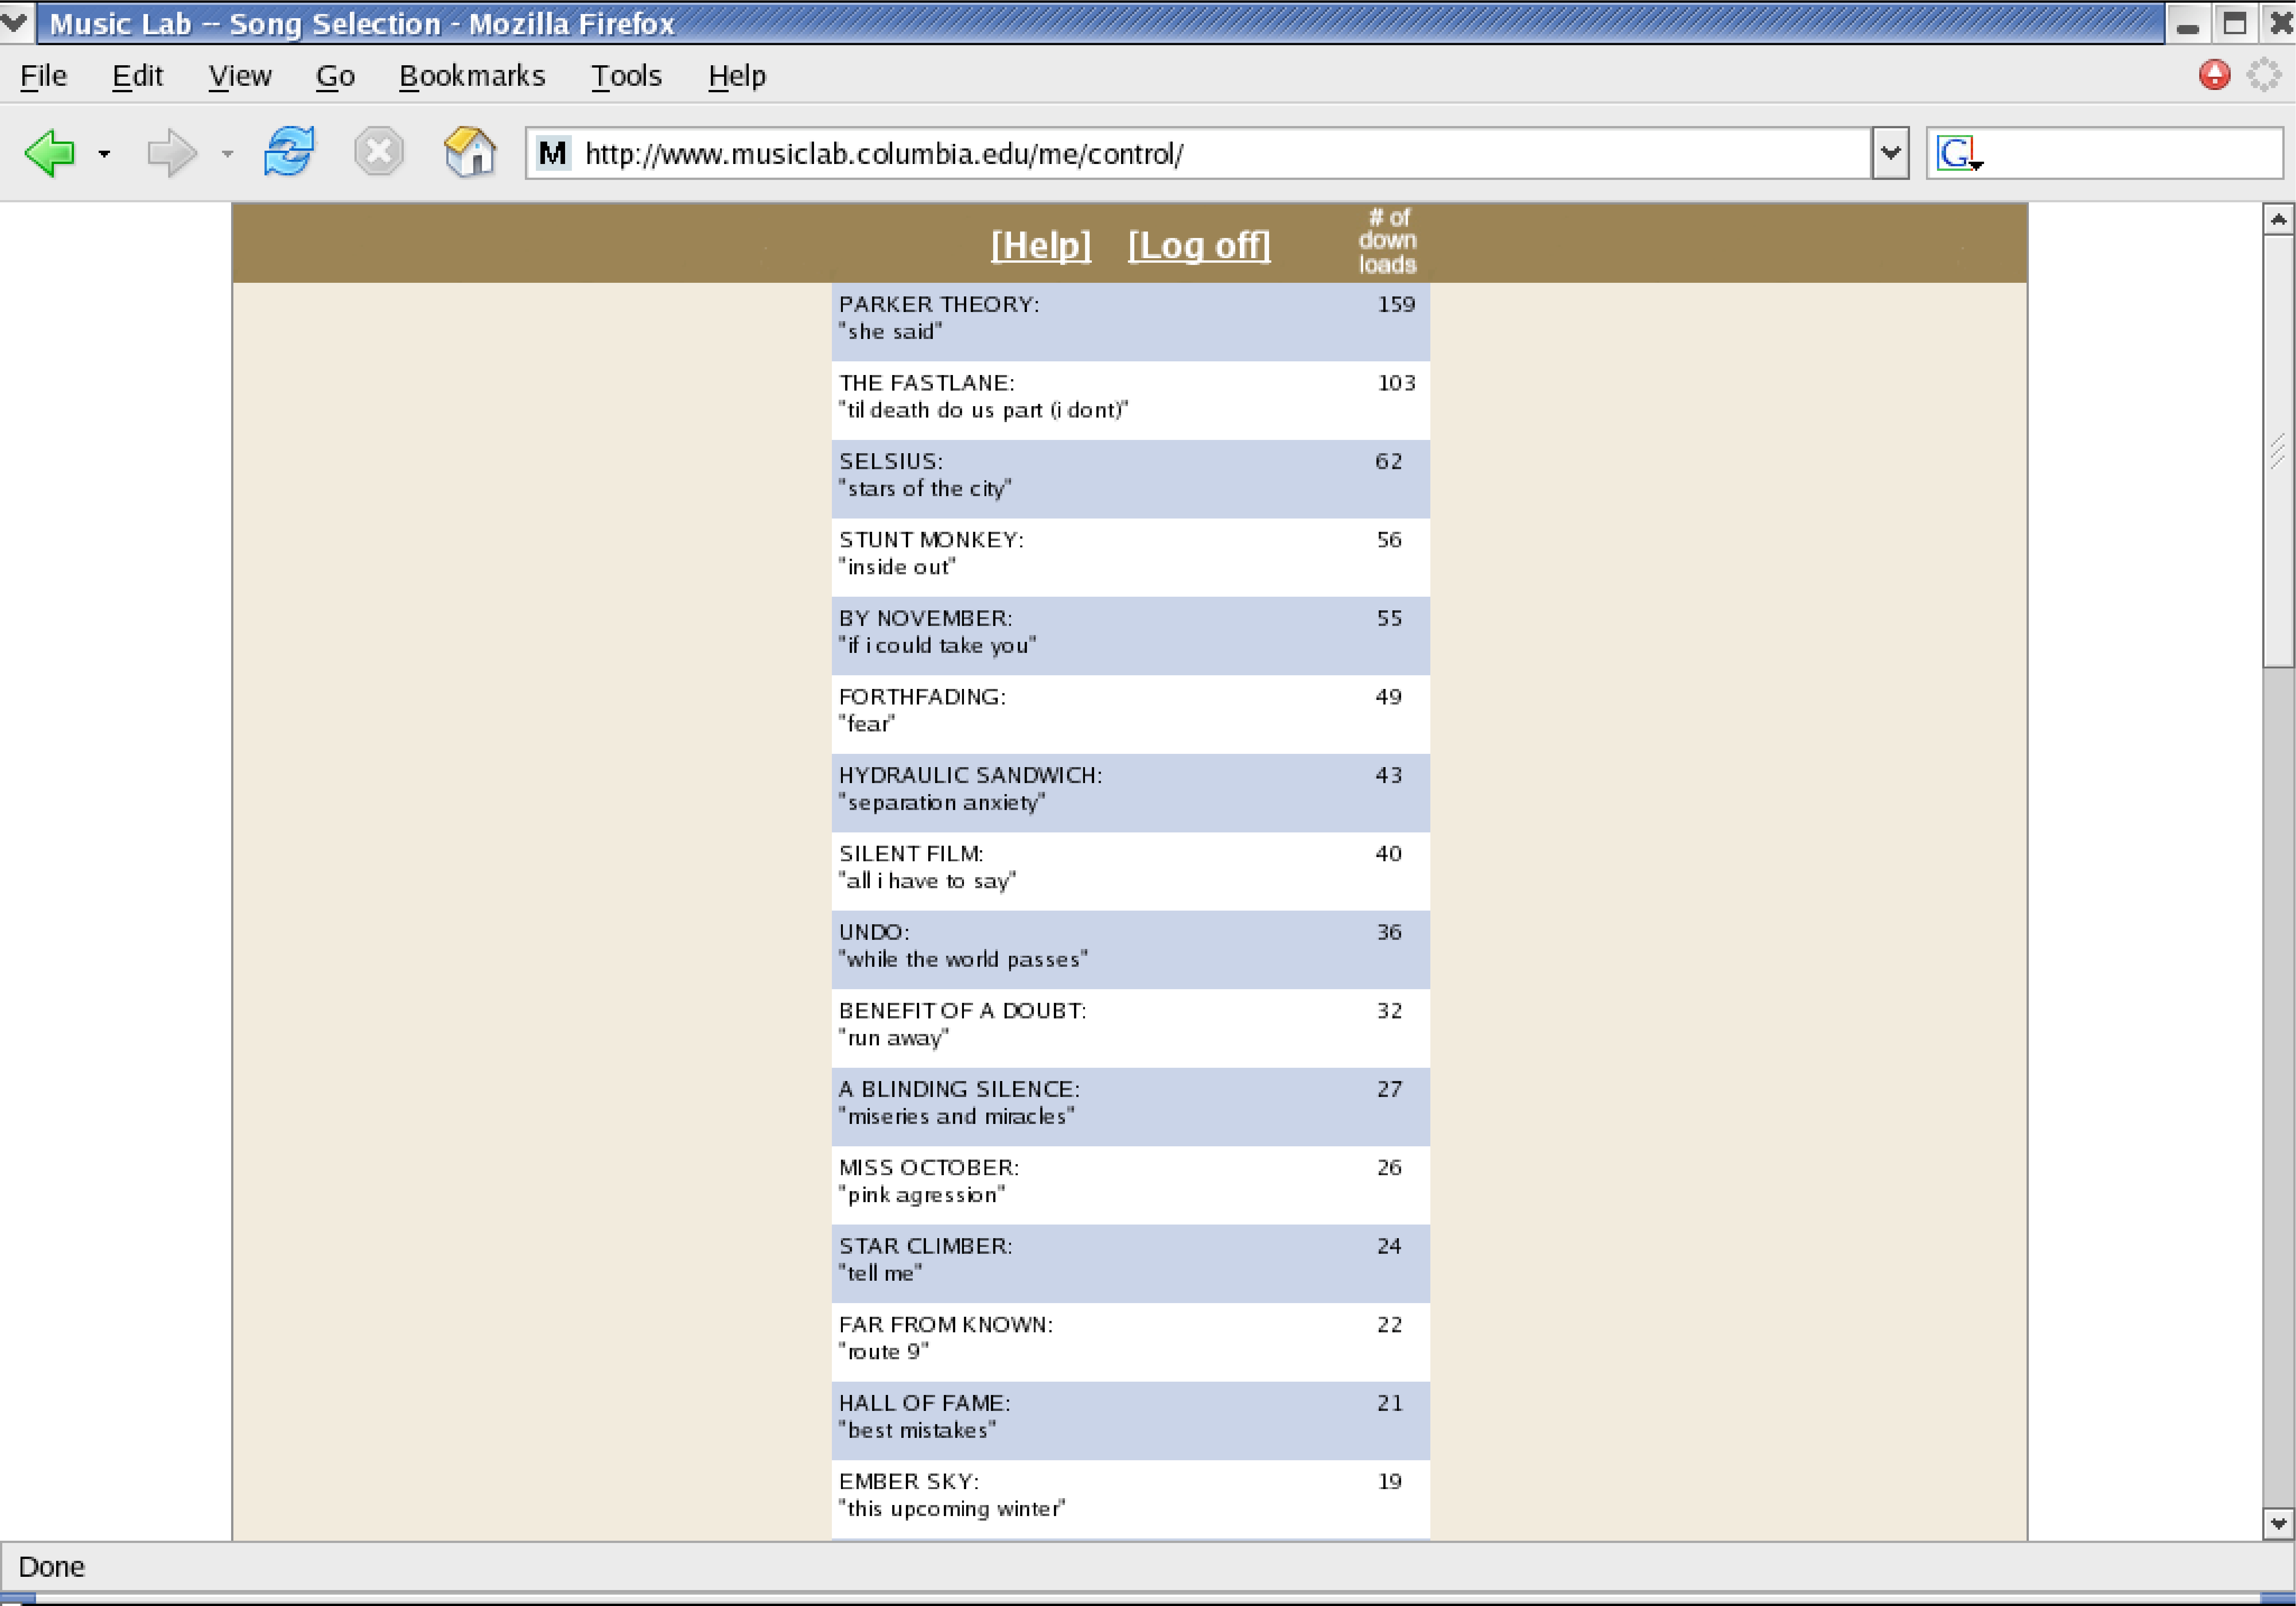
\includegraphics[width=0.45\textwidth]{figures/info-v2}}
\end{figure}

\end{frame}
%%%%%%%%%%%%%%%%%%%%%%%%%%%%%%
\begin{frame}

Reading notes:
\begin{itemize}
\item Notice the definition of unpredictability 
\pause
\item Looking at Fig 3 would you say the results are completely unpredictable?
\end{itemize}

\end{frame}
%%%%%%%%%%%%%%%%%%%%%%%%%%%%%
\begin{frame}

\begin{figure}
  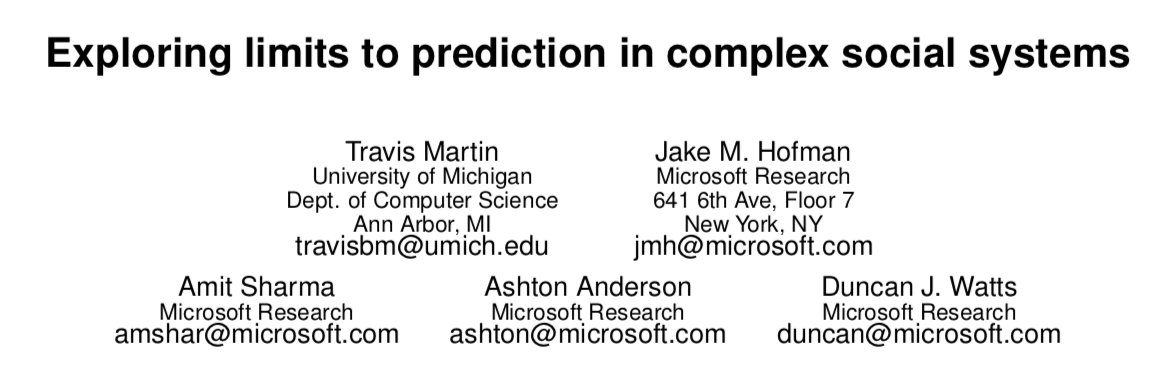
\includegraphics[width = 0.9\textwidth]{figures/martin_exploring_2016_title}
\end{figure}

\end{frame}
%%%%%%%%%%%%%%%%%%%%%%%%%%%%%
\begin{frame}

\begin{center}
\only<1>{
\includegraphics[width = 0.7\textwidth]{figures/arvind_tweet_nocount}}%
\only<2>{
\includegraphics[width = 0.7\textwidth]{figures/arvind_tweet_wcount}}%
\end{center}

\end{frame}
%%%%%%%%%%%%%%%%%%%%%%%%%%%%%
\begin{frame}

\begin{center}
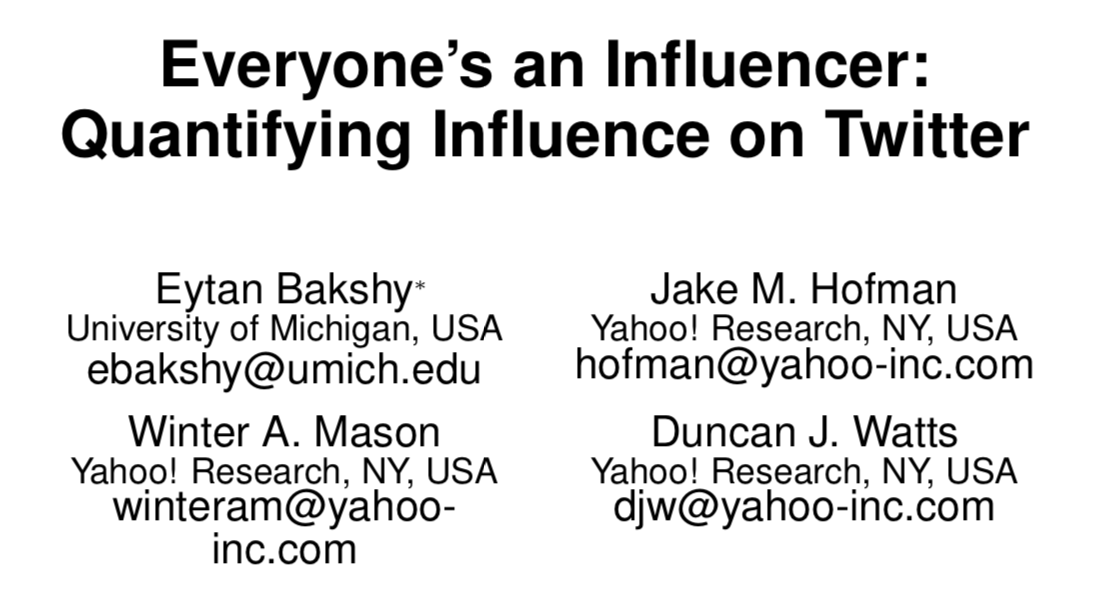
\includegraphics[width = 0.7\textwidth]{figures/bakshy_everyones_2011_title}
\end{center}

\end{frame}
%%%%%%%%%%%%%%%%%%%%%%%%%%%%%
\begin{frame}

\begin{itemize}
\item Lots of people write papers saying that they can predict retweets.
\pause
\item A skeptical reading of these papers raises questions.
\pause
\item Travis Martin tried to compare them and could not.
\end{itemize} 

\end{frame}
%%%%%%%%%%%%%%%%%%%%%%%%%%%%%
\begin{frame}

Reading notes:
\begin{itemize}
\item Ex-ante prediction vs ``peeking strategies''
\pause
\item Note how they choose to measure unpredictability.
\pause
\item stylized model, empirical results, reality-inspired simulation. What is the relationship between the empirical results and reality-inspired simulation?
\pause
\item Data generating process and measurement as fundamental sources of uncertainty.  Compare to ``War is in the Error'' term.
\pause
\item What is the fundamental limit and how close are we?
\pause
\item Is predicting re-tweets a setting where we think predictions should be successful? On the one hand lots of data. On the other hand, think of results from MusicLab.
\end{itemize} 

\end{frame}
%%%%%%%%%%%%%%%%%%%%%%%%%%%%%
\begin{frame}

\begin{center}
  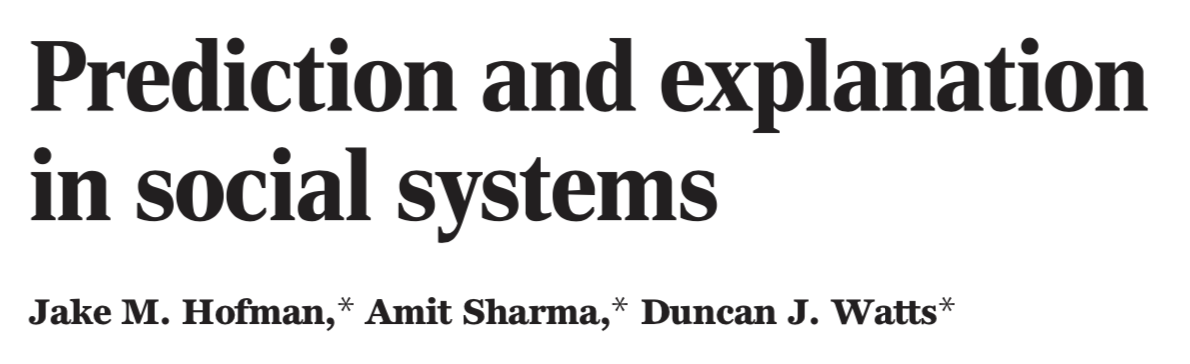
\includegraphics[width = 0.9\textwidth]{figures/hofman_prediction_2017_title}
\end{center}

\end{frame}
%%%%%%%%%%%%%%%%%%%%
\begin{frame}

Reading notes:
\begin{itemize}
\item Recall Brieman's two cultures.  This is related to the third way ``prediction for understanding''.
\pause
\item Argue for more careful way of evaluating predictions.
\pause
\item We should care about quantitatively finding fundamental limits to prediction whether we are computer scientist or social scientist.
\end{itemize} 

\end{frame}
%%%%%%%%%%%%%%%%%%%%%%%%%%%%%


\frame{\titlepage}


\end{document}
